\frame{\titlepage}
\frame{\frametitle{目录}\tableofcontents}

\section{“科文之争”}

\begin{frame}
  \frametitle{“科文之争”}

  \begin{itemize}
    \item \alert{十七年科幻}:受苏联“科学文艺”影响，此时国内科幻以科普为主，宣传社会主义，主要面向青少年
    \item \alert{黄金时期}(1978-1983):全国科学大会提出“向科学进军”，“科学热”引发了“科普热”、“科幻热”
    \item \alert{“科文之争”和“清污运动”}:科幻向姓“科”的血统发起的挑战
    \item \alert{90s之后科幻}:开始更多出现将科学幻想和哲学思考结合在一起的小说
  \end{itemize}
\end{frame}

\section{科幻给文学带来了什么}

\begin{frame}
  \frametitle{扩大了文学的描写空间}
  
  \alert{细节的巨大信息量}：科幻中的一个细节能包含上亿年的时间和上亿光年的空间
  \begin{itemize}
    \item \alert{《奇点焰火》}
    \item \alert{《星》} 阿瑟·克拉克：毁灭了一个文明的超新星，仅仅是为了照亮伯利恒的黎明！\footnote{“伯利恒的黎明”指圣经中记录的预示耶稣诞生的伯利恒之星。}
  
  \end{itemize}
  \vspace{0.4cm}
  \pause
  \alert{从描写个人到描写整个文明}：
  \begin{itemize}
    \item \alert{《最后的问题》} 阿西莫夫：从个人的发问到整个文明的发问
    \item \alert{《水晶天》} 大卫·布林
  \end{itemize}

\end{frame}

\begin{frame}
  \frametitle{社会的实验室}
  \begin{quoteBlock}{}
    科幻是作家用来考察人类社会，进行思想试验的实验室。—— 罗伯特·J·索耶
  \end{quoteBlock}

  科幻通过构建一个虚构的世界来探讨科学、道德、社会伦理等问题。在科幻中，现实世界的善恶好坏往往会被重新审视和定义。\pause
  \only<2>{    
    \begin{itemize}
      \item \alert{《三体Ⅱ：黑暗森林》} 刘慈欣：“一部分人死，或者所有人死。”
      \item \alert{《冷酷的方程式》} 汤姆·戈德温
  \end{itemize}
  }
  \pause
  \vspace{0.4cm}
  
  同时，在科幻中对社会道德等的探讨能展示未来可能出现的技术所产生的伦理问题。
  
  \begin{itemize}
    \item 《冷酷的方程式》中的类似于“电车难题”的道德困境与自动驾驶
    \item 基因编辑的伦理问题
  \end{itemize}
\end{frame}

\begin{frame}
  \frametitle{为想象提供新鲜血液}
  科学技术的发展本身也在扩充人类的想象力。如果没有科学，$460$ 亿光年和 $10^{-18}$ 米只是疯子的呓语。人类的想象世界借助科学的发展扩充了数倍。

  \begin{minipage}[t]{0.6\textwidth}
    \begin{figure}[htpb]
      \centering
      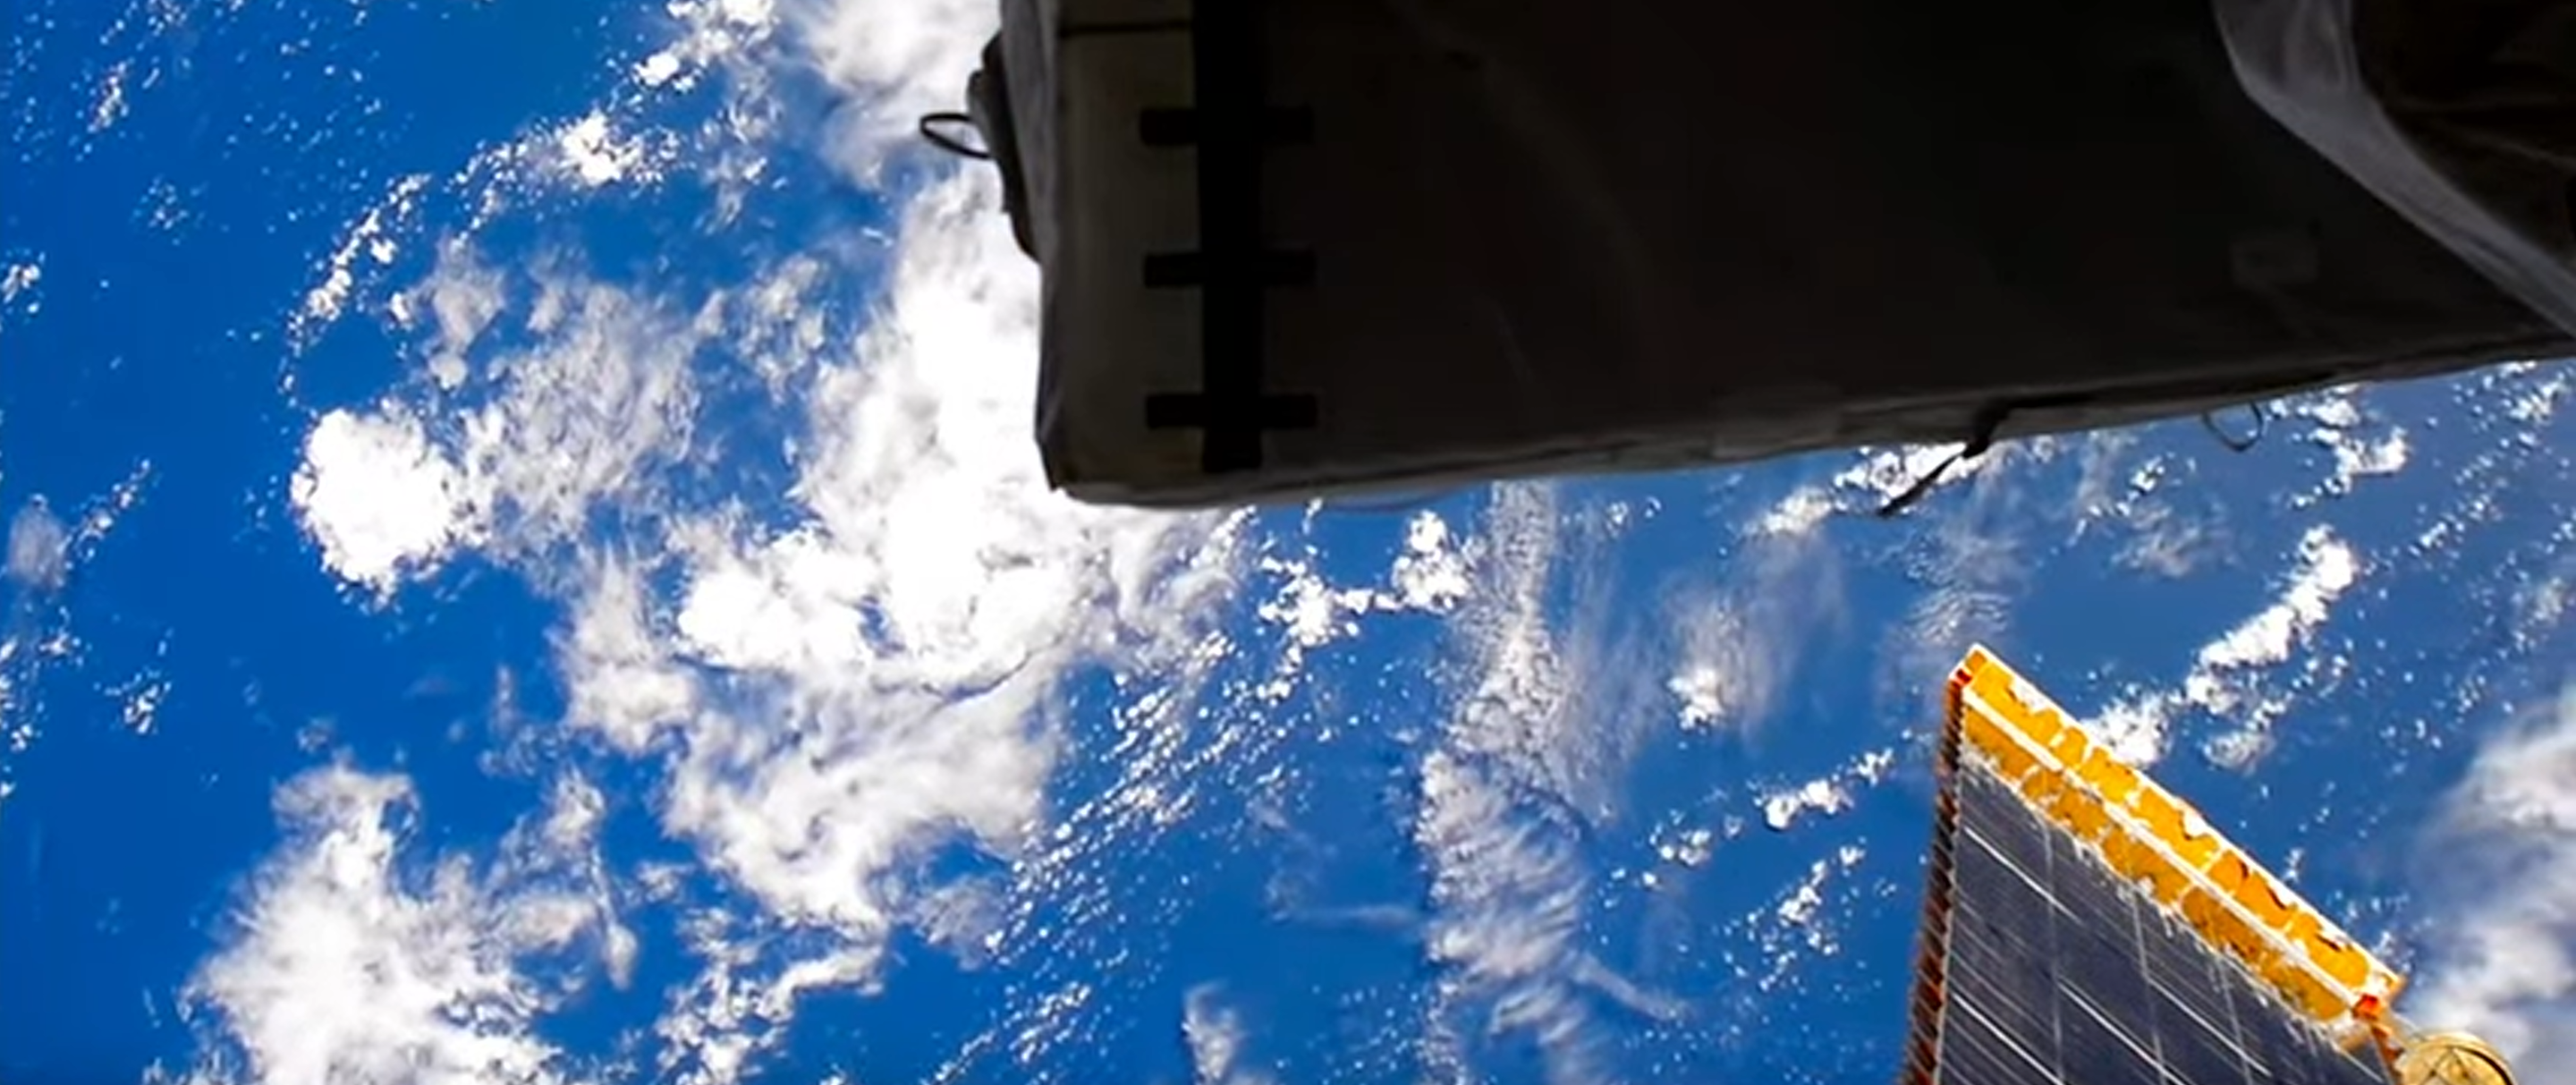
\includegraphics[height=0.45\textheight]{./imgs/ISS.png}
      \caption{ISS 直播截图}
    \end{figure}
  \end{minipage}
  \hfill
  \begin{minipage}[t]{0.38\textwidth}
    \begin{figure}[htpb]
      \centering
      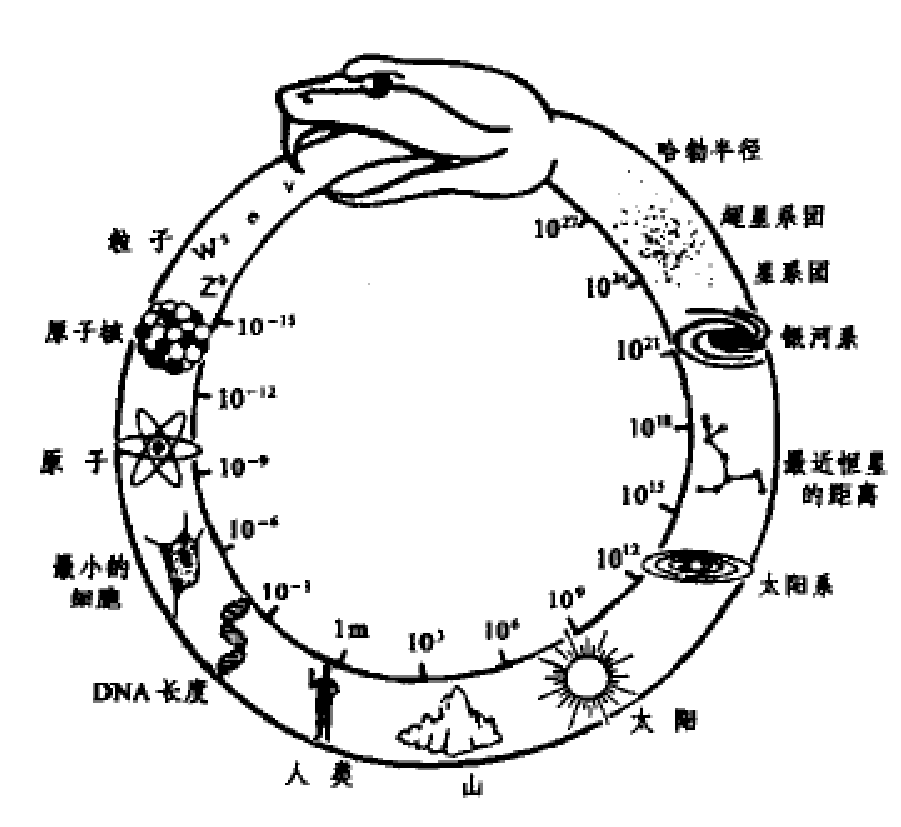
\includegraphics[height=0.45\textheight]{./imgs/S.png}
      \caption{极大与极小}
    \end{figure}
  \end{minipage}

\end{frame}

\begin{frame}
  \frametitle{探讨人与自然、人与技术的关系}
  科幻不止讨论人与人的关系，还探讨了人与自然、人与技术的关系。在科幻作品中，自然和技术本身也是和人同样重要的主人公
  
  \vspace{0.4cm}
  
  \begin{minipage}[c]{0.5\textwidth}
  \begin{itemize}
    \item \alert{《2001：太空漫游》} 阿瑟·克拉克
    \item \alert{《被遗忘的敌人》} 阿瑟·克拉克
    \item \alert{《宇宙墓碑》} 韩松
  \end{itemize}
  \end{minipage}
  \hfill
  \begin{minipage}[c]{0.45\textwidth}
    \begin{noteBlock}
      在此类作品中表达的不是征人对自然的征服，而是描述对自然既好奇又敬畏、既热爱又恐惧的情感
    \end{noteBlock}
  \end{minipage}
  
  \vspace{0.4cm}

  同时，在对人与自然的讨论中，我们重新审视了人类自身的地位
  
  \begin{itemize}
    \item \alert{《路边野餐》} 阿卡迪·斯特鲁伽茨基：颠覆以人类中心的理论
  \end{itemize}
\end{frame}

\section{科幻与科学}

\begin{frame}
  \frametitle{科幻能展示科学中的美}
  在科幻中，我们会惊叹于其中绝妙的点子，其中有一些本身就是科学中的绝妙的想法。只是科学中的想法很多被高深艰涩的数学或者前置知识所隐藏，使得读者难以体会。而科幻向我们展示其中的一部分（虽然有所简化），从而激发起人们的科学兴趣。
  
  \vspace{0.4cm}

  \begin{itemize}
    \item \alert{分析力学}：不需要“力”的力学
    \item \alert{诺特定理}：一个守恒量对应一个对称性
    \item \alert{化学渗透}：二十世纪最“反直觉”的生物发现
  \end{itemize}
  \vspace{0.4cm}
\end{frame}

\begin{frame}
  \frametitle{科幻中科学错误的分类}
  科幻作者很多时候并不是这个领域的专家，科幻作品也并不一定符合目前已知的科学理论。
  
  %\vspace{0.4cm}
  \only<1>{
    \vspace{0.4cm}
    
    \begin{block}{一些例外}
      \begin{itemize}
      \item \alert{《真空态》} 杰弗里·兰迪斯：“对称性破缺”（过冷水与爆炸性结晶）
      \item \alert{《龙蛋》} 罗伯特·福沃德：“一本伪装成小说的中子星教科书”
    \end{itemize}
    \end{block}
    
    \vspace{0.4cm}

    实际上科幻写作有时并不需要了解前沿科学的具体原理。假设小说中要描写一个运行大量“数字生命”的计算机集群，相比于具体的计算机程序设计等内容，了解计算机集群的运行场景可能更为重要。
  }
  \pause
  
  可以说科幻作品中的科学错误是难以避免的。刘慈欣曾经将科幻小说中的硬伤分为下面四种：
  \begin{itemize}
    \item \alert{疏忽硬伤}：作者一时疏忽出现的硬伤
    \item \alert{知识硬伤}：由于作者的知识水平所限所出现的硬伤 （刘慈欣《鲸歌》：蓝鲸长出牙齿）
    \item \alert{背景硬伤}：硬伤是故事赖以生存的条件（刘慈欣《流浪地球》：推动地球）
    \item \alert{灵魂硬伤}：硬伤本身就是小说中最独特的地方，硬伤就是这类科幻的灵魂
  \end{itemize}

\end{frame}

\begin{frame}
  \frametitle{灵魂硬伤：最高级的科幻}
  在这类科幻小说中，其幻想了一个和目前物理规律不同的世界，并探讨在这个世界中会发生什么？
  \begin{itemize}
    \item \alert{《TSIAL星球的悲剧》}（又名《重冰》）G·R·尤赫：冰的密度大于水
    \item \alert{《三体Ⅲ：死神永生》} 刘慈欣：低光速黑域
    \item 修改万有引力定律（$F = G \frac{Mm}{r^n}$，$n = 3$ 或等于其他）
  \end{itemize}

  \begin{minipage}[t]{0.55\linewidth}
    \begin{block}{Bertrand 定理}
      当且仅当 $n=2$ 或 $n=-1$ 时才有稳定轨道。
    \end{block}
  \end{minipage}
  \hfill
  \begin{minipage}[t]{0.21\linewidth}
    \begin{figure}[htpb]
      \centering
      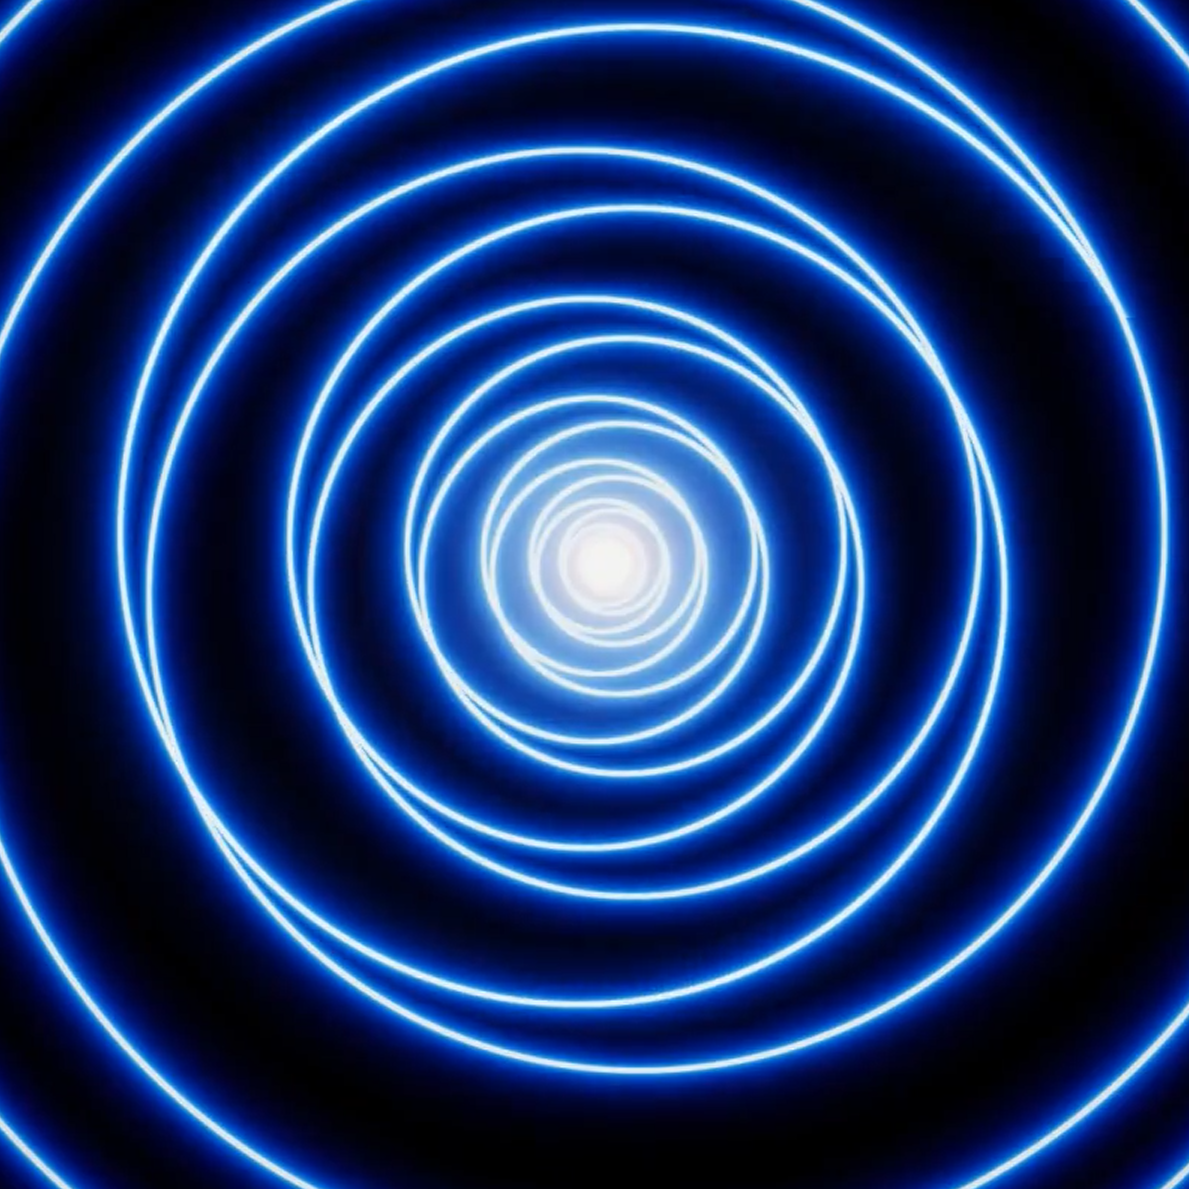
\includegraphics[width=0.8\textwidth]{./imgs/n3.png}
      \caption{$n=3$}
    \end{figure}
  \end{minipage}
  \hfill
  \begin{minipage}[t]{0.21\linewidth}
    \begin{figure}[htpb]
      \centering
      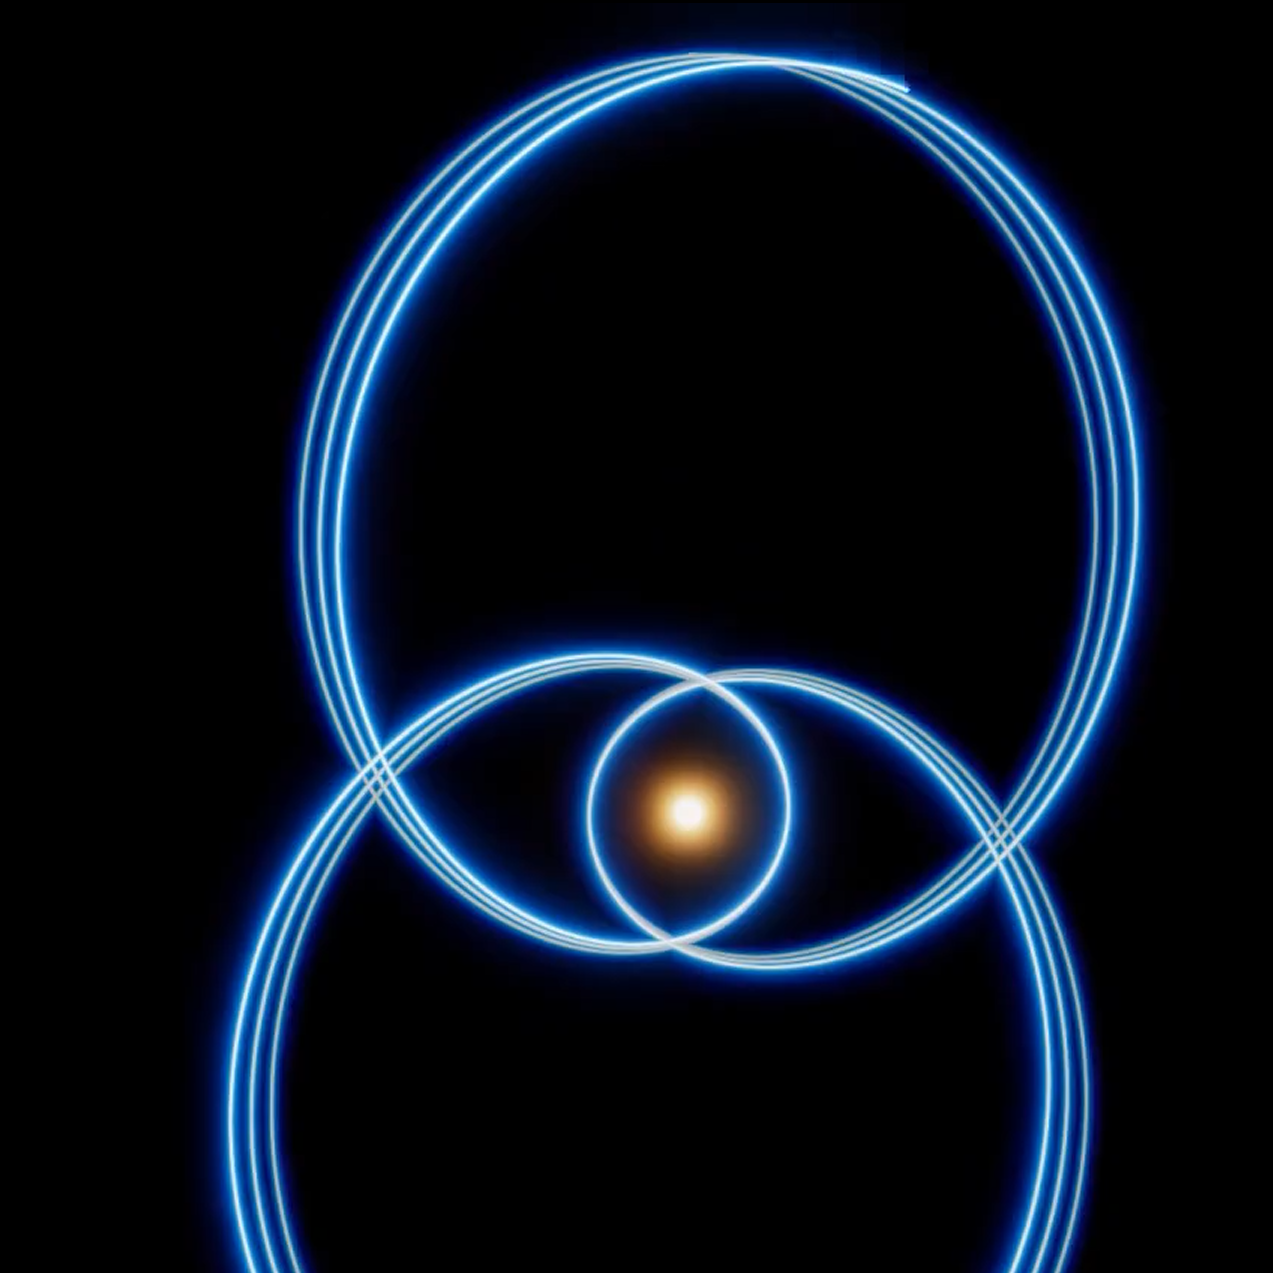
\includegraphics[width=0.8\textwidth]{./imgs/n25.png}
      \caption{$n=2.5$}
    \end{figure}
  \end{minipage}

\end{frame}

\section{尾声}

\begin{frame}{尾声}
  \begin{center}
    \Huge Thanks!
  \end{center}
  \begin{quoteBlock}
    任何二元论都有可能将问题简化
  \end{quoteBlock}
  \begin{quoteBlock}
    科普型科幻是中国的创造，而中国科幻最大的辉煌也是科普型科幻创造的……科幻是姓文还是姓科，其实全无意义，为什么不能一部分姓文一部分姓科呢？——刘慈欣
  \end{quoteBlock}
\end{frame}
